\batchmode
\documentclass[a4paper]{book}
\usepackage{makeidx}
\usepackage{graphicx}
\usepackage{multicol}
\usepackage{float}
\usepackage{listings}
\usepackage{color}
\usepackage{ifthen}
\usepackage[table]{xcolor}
\usepackage{textcomp}
\usepackage{alltt}
\usepackage[utf8]{inputenc}
\usepackage{mathptmx}
\usepackage[scaled=.90]{helvet}
\usepackage{courier}
\usepackage{sectsty}
\usepackage[titles]{tocloft}
\usepackage{doxygen}
\lstset{language=C++,inputencoding=utf8,basicstyle=\footnotesize,breaklines=true,breakatwhitespace=true,tabsize=8,numbers=left }
\makeindex
\setcounter{tocdepth}{3}
\renewcommand{\footrulewidth}{0.4pt}
\renewcommand{\familydefault}{\sfdefault}
\begin{document}
\begin{titlepage}
\vspace*{7cm}
\begin{center}
{\Large teleop\_\-source\_\-keyboard }\\
\vspace*{1cm}
{\large Generated by Doxygen 1.7.4}\\
\vspace*{0.5cm}
{\small Sun Feb 26 2012 08:45:59}\\
\end{center}
\end{titlepage}
\clearemptydoublepage
\pagenumbering{roman}
\tableofcontents
\clearemptydoublepage
\pagenumbering{arabic}
\chapter{Main Page}
\label{index} 
\chapter{Namespace Index}
\section{Namespace List}
Here is a list of all namespaces with brief descriptions:\begin{DoxyCompactList}
\item\contentsline{section}{{\bf ros} }{\pageref{namespaceros}}{}
\item\contentsline{section}{{\bf ros::message\_\-operations} }{\pageref{namespaceros_1_1message__operations}}{}
\item\contentsline{section}{{\bf ros::message\_\-traits} }{\pageref{namespaceros_1_1message__traits}}{}
\item\contentsline{section}{{\bf ros::serialization} }{\pageref{namespaceros_1_1serialization}}{}
\item\contentsline{section}{{\bf teleop\_\-msgs} }{\pageref{namespaceteleop__msgs}}{}
\item\contentsline{section}{{\bf teleop\_\-msgs::msg} }{\pageref{namespaceteleop__msgs_1_1msg}}{}
\item\contentsline{section}{{\bf teleop\_\-msgs::msg::\_\-Axis} }{\pageref{namespaceteleop__msgs_1_1msg_1_1__Axis}}{}
\item\contentsline{section}{{\bf teleop\_\-msgs::msg::\_\-Button} }{\pageref{namespaceteleop__msgs_1_1msg_1_1__Button}}{}
\item\contentsline{section}{{\bf teleop\_\-msgs::msg::\_\-State} }{\pageref{namespaceteleop__msgs_1_1msg_1_1__State}}{}
\end{DoxyCompactList}

\chapter{Class Index}
\section{Class List}
Here are the classes, structs, unions and interfaces with brief descriptions:\begin{DoxyCompactList}
\item\contentsline{section}{{\bf teleop::TeleopSourceJoystick} }{\pageref{classteleop_1_1TeleopSourceJoystick}}{}
\end{DoxyCompactList}

\chapter{File Index}
\section{File List}
Here is a list of all files with brief descriptions:\begin{DoxyCompactList}
\item\contentsline{section}{/home/klc/Code/github.com/teleop/teleop\_\-msgs/msg\_\-gen/cpp/include/teleop\_\-msgs/{\bf Axis.h} }{\pageref{Axis_8h}}{}
\item\contentsline{section}{/home/klc/Code/github.com/teleop/teleop\_\-msgs/msg\_\-gen/cpp/include/teleop\_\-msgs/{\bf Button.h} }{\pageref{Button_8h}}{}
\item\contentsline{section}{/home/klc/Code/github.com/teleop/teleop\_\-msgs/msg\_\-gen/cpp/include/teleop\_\-msgs/{\bf State.h} }{\pageref{State_8h}}{}
\item\contentsline{section}{/home/klc/Code/github.com/teleop/teleop\_\-msgs/src/teleop\_\-msgs/{\bf \_\-\_\-init\_\-\_\-.py} }{\pageref{____init_____8py}}{}
\item\contentsline{section}{/home/klc/Code/github.com/teleop/teleop\_\-msgs/src/teleop\_\-msgs/msg/{\bf \_\-\_\-init\_\-\_\-.py} }{\pageref{msg_2____init_____8py}}{}
\item\contentsline{section}{/home/klc/Code/github.com/teleop/teleop\_\-msgs/src/teleop\_\-msgs/msg/{\bf \_\-Axis.py} }{\pageref{__Axis_8py}}{}
\item\contentsline{section}{/home/klc/Code/github.com/teleop/teleop\_\-msgs/src/teleop\_\-msgs/msg/{\bf \_\-Button.py} }{\pageref{__Button_8py}}{}
\item\contentsline{section}{/home/klc/Code/github.com/teleop/teleop\_\-msgs/src/teleop\_\-msgs/msg/{\bf \_\-State.py} }{\pageref{__State_8py}}{}
\end{DoxyCompactList}

\chapter{Namespace Documentation}
\section{teleop Namespace Reference}
\label{namespaceteleop}\index{teleop@{teleop}}
\subsection*{Classes}
\begin{DoxyCompactItemize}
\item 
class {\bf TeleopSourceJoystick}
\end{DoxyCompactItemize}

\chapter{Class Documentation}
\section{teleop::TeleopSourceKeyboard Class Reference}
\label{classteleop_1_1TeleopSourceKeyboard}\index{teleop::TeleopSourceKeyboard@{teleop::TeleopSourceKeyboard}}


{\ttfamily \#include $<$teleop\_\-source\_\-keyboard.hpp$>$}

\subsection*{Public Member Functions}
\begin{DoxyCompactItemize}
\item 
unsigned int {\bf getSteps} ()
\item 
virtual bool {\bf init} ()
\item 
virtual bool {\bf listen} (unsigned int listenTimeout, TeleopState $\ast$const teleopState, bool $\ast$updated)
\item 
bool {\bf setSteps} (unsigned int steps)
\item 
virtual bool {\bf shutdown} ()
\item 
{\bf TeleopSourceKeyboard} ()
\item 
{\bf $\sim$TeleopSourceKeyboard} ()
\end{DoxyCompactItemize}
\subsection*{Static Public Attributes}
\paragraph*{}
\begin{DoxyCompactItemize}
\item 
static const unsigned int {\bf STEPS\_\-DEFAULT} = 3
\item 
static const unsigned int {\bf STEPS\_\-MIN} = 1
\item 
static const unsigned int {\bf STEPS\_\-MAX} = 5
\end{DoxyCompactItemize}

\subsection*{Private Member Functions}
\begin{DoxyCompactItemize}
\item 
bool {\bf handleEvent} (char c, TeleopState $\ast$const teleopState, bool $\ast$updated)
\end{DoxyCompactItemize}
\subsection*{Private Attributes}
\begin{DoxyCompactItemize}
\item 
bool {\bf mIsInitialised}
\item 
boost::recursive\_\-mutex {\bf mMemberMutex}
\item 
struct termios {\bf mOldTermios}
\item 
unsigned int {\bf mSteps}
\item 
TeleopAxisValue {\bf mStepSize}
\end{DoxyCompactItemize}
\subsection*{Static Private Attributes}
\paragraph*{}
\begin{DoxyCompactItemize}
\item 
static const unsigned int {\bf KEYCODE\_\-SPACE} = 0x20
\item 
static const unsigned int {\bf KEYCODE\_\-UP} = 0x41
\item 
static const unsigned int {\bf KEYCODE\_\-DOWN} = 0x42
\item 
static const unsigned int {\bf KEYCODE\_\-RIGHT} = 0x43
\item 
static const unsigned int {\bf KEYCODE\_\-LEFT} = 0x44
\end{DoxyCompactItemize}



\subsection{Detailed Description}
This class implements a keyboard teleop source. The arrow keys are used to increment and decrement the linear X and Y axes relative to the previous teleop source state, which is passed into the listen method. The space bar acts as a stop button.

Key presses are detected by reading raw standard input using termios. If this class is used, other uses of standard input from within the same process should be handled carefully. This approach should be fairly portable, and it doesn't require a graphical environment or low-\/level operating system inputs. 

Definition at line 74 of file teleop\_\-source\_\-keyboard.hpp.



\subsection{Constructor \& Destructor Documentation}
\index{teleop::TeleopSourceKeyboard@{teleop::TeleopSourceKeyboard}!TeleopSourceKeyboard@{TeleopSourceKeyboard}}
\index{TeleopSourceKeyboard@{TeleopSourceKeyboard}!teleop::TeleopSourceKeyboard@{teleop::TeleopSourceKeyboard}}
\subsubsection[{TeleopSourceKeyboard}]{\setlength{\rightskip}{0pt plus 5cm}teleop::TeleopSourceKeyboard::TeleopSourceKeyboard (
\begin{DoxyParamCaption}
{}
\end{DoxyParamCaption}
)}\label{classteleop_1_1TeleopSourceKeyboard_a0507ac337a50bcfbbb82bc7519d3e071}
Constructor. 

Definition at line 74 of file teleop\_\-source\_\-keyboard.cpp.

\index{teleop::TeleopSourceKeyboard@{teleop::TeleopSourceKeyboard}!$\sim$TeleopSourceKeyboard@{$\sim$TeleopSourceKeyboard}}
\index{$\sim$TeleopSourceKeyboard@{$\sim$TeleopSourceKeyboard}!teleop::TeleopSourceKeyboard@{teleop::TeleopSourceKeyboard}}
\subsubsection[{$\sim$TeleopSourceKeyboard}]{\setlength{\rightskip}{0pt plus 5cm}teleop::TeleopSourceKeyboard::$\sim$TeleopSourceKeyboard (
\begin{DoxyParamCaption}
{}
\end{DoxyParamCaption}
)}\label{classteleop_1_1TeleopSourceKeyboard_a30ef4fbadec4e60b35d758c105101c12}
Destructor. 

Definition at line 80 of file teleop\_\-source\_\-keyboard.cpp.



\subsection{Member Function Documentation}
\index{teleop::TeleopSourceKeyboard@{teleop::TeleopSourceKeyboard}!getSteps@{getSteps}}
\index{getSteps@{getSteps}!teleop::TeleopSourceKeyboard@{teleop::TeleopSourceKeyboard}}
\subsubsection[{getSteps}]{\setlength{\rightskip}{0pt plus 5cm}unsigned int teleop::TeleopSourceKeyboard::getSteps (
\begin{DoxyParamCaption}
{}
\end{DoxyParamCaption}
)}\label{classteleop_1_1TeleopSourceKeyboard_acafb24af4e321d318fb23ad86a27841e}
Get the number of steps required to reach the maximum value for all axes.

\begin{DoxyReturn}{Returns}
steps 
\end{DoxyReturn}


Definition at line 105 of file teleop\_\-source\_\-keyboard.cpp.

\index{teleop::TeleopSourceKeyboard@{teleop::TeleopSourceKeyboard}!handleEvent@{handleEvent}}
\index{handleEvent@{handleEvent}!teleop::TeleopSourceKeyboard@{teleop::TeleopSourceKeyboard}}
\subsubsection[{handleEvent}]{\setlength{\rightskip}{0pt plus 5cm}bool teleop::TeleopSourceKeyboard::handleEvent (
\begin{DoxyParamCaption}
\item[{char}]{c, }
\item[{TeleopState $\ast$const}]{teleopState, }
\item[{bool $\ast$}]{updated}
\end{DoxyParamCaption}
)\hspace{0.3cm}{\ttfamily  [private]}}\label{classteleop_1_1TeleopSourceKeyboard_acf67e84c454aaa19fe4adb0ec6292181}
Handle a given event.


\begin{DoxyParams}{Parameters}
{\em c} & [in] -\/ character to handle \\
\hline
{\em teleopState} & [in/out] -\/ the current teleop state, to be updated \\
\hline
{\em updated} & [in/out] -\/ true if teleop state was updated\\
\hline
\end{DoxyParams}
\begin{DoxyReturn}{Returns}
true on success 
\end{DoxyReturn}


Definition at line 226 of file teleop\_\-source\_\-keyboard.cpp.

\index{teleop::TeleopSourceKeyboard@{teleop::TeleopSourceKeyboard}!init@{init}}
\index{init@{init}!teleop::TeleopSourceKeyboard@{teleop::TeleopSourceKeyboard}}
\subsubsection[{init}]{\setlength{\rightskip}{0pt plus 5cm}bool teleop::TeleopSourceKeyboard::init (
\begin{DoxyParamCaption}
{}
\end{DoxyParamCaption}
)\hspace{0.3cm}{\ttfamily  [virtual]}}\label{classteleop_1_1TeleopSourceKeyboard_acb6dc7945969ccae2c4f51c8f96c8b24}
Override virtual method from parent. 

Definition at line 113 of file teleop\_\-source\_\-keyboard.cpp.

\index{teleop::TeleopSourceKeyboard@{teleop::TeleopSourceKeyboard}!listen@{listen}}
\index{listen@{listen}!teleop::TeleopSourceKeyboard@{teleop::TeleopSourceKeyboard}}
\subsubsection[{listen}]{\setlength{\rightskip}{0pt plus 5cm}bool teleop::TeleopSourceKeyboard::listen (
\begin{DoxyParamCaption}
\item[{unsigned int}]{listenTimeout, }
\item[{TeleopState $\ast$const}]{teleopState, }
\item[{bool $\ast$}]{updated}
\end{DoxyParamCaption}
)\hspace{0.3cm}{\ttfamily  [virtual]}}\label{classteleop_1_1TeleopSourceKeyboard_a6db4e5b72630d453e8c83eb344a957a0}
Override virtual method from parent. 

Definition at line 143 of file teleop\_\-source\_\-keyboard.cpp.

\index{teleop::TeleopSourceKeyboard@{teleop::TeleopSourceKeyboard}!setSteps@{setSteps}}
\index{setSteps@{setSteps}!teleop::TeleopSourceKeyboard@{teleop::TeleopSourceKeyboard}}
\subsubsection[{setSteps}]{\setlength{\rightskip}{0pt plus 5cm}bool teleop::TeleopSourceKeyboard::setSteps (
\begin{DoxyParamCaption}
\item[{unsigned int}]{steps}
\end{DoxyParamCaption}
)}\label{classteleop_1_1TeleopSourceKeyboard_a28995ad18ec315458a066c30fd94b76a}
Set the number of steps required to reach the maximum value for all axes.


\begin{DoxyParams}{Parameters}
{\em steps} & [in] -\/ number of steps\\
\hline
\end{DoxyParams}
\begin{DoxyReturn}{Returns}
true on success 
\end{DoxyReturn}


Definition at line 87 of file teleop\_\-source\_\-keyboard.cpp.

\index{teleop::TeleopSourceKeyboard@{teleop::TeleopSourceKeyboard}!shutdown@{shutdown}}
\index{shutdown@{shutdown}!teleop::TeleopSourceKeyboard@{teleop::TeleopSourceKeyboard}}
\subsubsection[{shutdown}]{\setlength{\rightskip}{0pt plus 5cm}bool teleop::TeleopSourceKeyboard::shutdown (
\begin{DoxyParamCaption}
{}
\end{DoxyParamCaption}
)\hspace{0.3cm}{\ttfamily  [virtual]}}\label{classteleop_1_1TeleopSourceKeyboard_ac238622c5e702be5b778132918877e9b}
Override virtual method from parent. 

Definition at line 206 of file teleop\_\-source\_\-keyboard.cpp.



\subsection{Member Data Documentation}
\index{teleop::TeleopSourceKeyboard@{teleop::TeleopSourceKeyboard}!KEYCODE\_\-DOWN@{KEYCODE\_\-DOWN}}
\index{KEYCODE\_\-DOWN@{KEYCODE\_\-DOWN}!teleop::TeleopSourceKeyboard@{teleop::TeleopSourceKeyboard}}
\subsubsection[{KEYCODE\_\-DOWN}]{\setlength{\rightskip}{0pt plus 5cm}const unsigned int {\bf teleop::TeleopSourceKeyboard::KEYCODE\_\-DOWN} = 0x42\hspace{0.3cm}{\ttfamily  [static, private]}}\label{classteleop_1_1TeleopSourceKeyboard_abe548a06d67edb0f75672ee2d386cdfc}


Definition at line 130 of file teleop\_\-source\_\-keyboard.hpp.

\index{teleop::TeleopSourceKeyboard@{teleop::TeleopSourceKeyboard}!KEYCODE\_\-LEFT@{KEYCODE\_\-LEFT}}
\index{KEYCODE\_\-LEFT@{KEYCODE\_\-LEFT}!teleop::TeleopSourceKeyboard@{teleop::TeleopSourceKeyboard}}
\subsubsection[{KEYCODE\_\-LEFT}]{\setlength{\rightskip}{0pt plus 5cm}const unsigned int {\bf teleop::TeleopSourceKeyboard::KEYCODE\_\-LEFT} = 0x44\hspace{0.3cm}{\ttfamily  [static, private]}}\label{classteleop_1_1TeleopSourceKeyboard_afbed9335a8e3178b1e231700e3bd9439}


Definition at line 132 of file teleop\_\-source\_\-keyboard.hpp.

\index{teleop::TeleopSourceKeyboard@{teleop::TeleopSourceKeyboard}!KEYCODE\_\-RIGHT@{KEYCODE\_\-RIGHT}}
\index{KEYCODE\_\-RIGHT@{KEYCODE\_\-RIGHT}!teleop::TeleopSourceKeyboard@{teleop::TeleopSourceKeyboard}}
\subsubsection[{KEYCODE\_\-RIGHT}]{\setlength{\rightskip}{0pt plus 5cm}const unsigned int {\bf teleop::TeleopSourceKeyboard::KEYCODE\_\-RIGHT} = 0x43\hspace{0.3cm}{\ttfamily  [static, private]}}\label{classteleop_1_1TeleopSourceKeyboard_a9bfab5df9ab3df814bf7ce6ab39e0623}


Definition at line 131 of file teleop\_\-source\_\-keyboard.hpp.

\index{teleop::TeleopSourceKeyboard@{teleop::TeleopSourceKeyboard}!KEYCODE\_\-SPACE@{KEYCODE\_\-SPACE}}
\index{KEYCODE\_\-SPACE@{KEYCODE\_\-SPACE}!teleop::TeleopSourceKeyboard@{teleop::TeleopSourceKeyboard}}
\subsubsection[{KEYCODE\_\-SPACE}]{\setlength{\rightskip}{0pt plus 5cm}const unsigned int {\bf teleop::TeleopSourceKeyboard::KEYCODE\_\-SPACE} = 0x20\hspace{0.3cm}{\ttfamily  [static, private]}}\label{classteleop_1_1TeleopSourceKeyboard_aaeaf99220d79f9b4221efb4cdfd27f80}
Keycodes 

Definition at line 128 of file teleop\_\-source\_\-keyboard.hpp.

\index{teleop::TeleopSourceKeyboard@{teleop::TeleopSourceKeyboard}!KEYCODE\_\-UP@{KEYCODE\_\-UP}}
\index{KEYCODE\_\-UP@{KEYCODE\_\-UP}!teleop::TeleopSourceKeyboard@{teleop::TeleopSourceKeyboard}}
\subsubsection[{KEYCODE\_\-UP}]{\setlength{\rightskip}{0pt plus 5cm}const unsigned int {\bf teleop::TeleopSourceKeyboard::KEYCODE\_\-UP} = 0x41\hspace{0.3cm}{\ttfamily  [static, private]}}\label{classteleop_1_1TeleopSourceKeyboard_a4da8566192b9c90e07f9bc1bf283d1d4}


Definition at line 129 of file teleop\_\-source\_\-keyboard.hpp.

\index{teleop::TeleopSourceKeyboard@{teleop::TeleopSourceKeyboard}!mIsInitialised@{mIsInitialised}}
\index{mIsInitialised@{mIsInitialised}!teleop::TeleopSourceKeyboard@{teleop::TeleopSourceKeyboard}}
\subsubsection[{mIsInitialised}]{\setlength{\rightskip}{0pt plus 5cm}bool {\bf teleop::TeleopSourceKeyboard::mIsInitialised}\hspace{0.3cm}{\ttfamily  [private]}}\label{classteleop_1_1TeleopSourceKeyboard_a83ec820735c831ac44344094548a7ccf}
Flag indicating if we are prepared to listen 

Definition at line 139 of file teleop\_\-source\_\-keyboard.hpp.

\index{teleop::TeleopSourceKeyboard@{teleop::TeleopSourceKeyboard}!mMemberMutex@{mMemberMutex}}
\index{mMemberMutex@{mMemberMutex}!teleop::TeleopSourceKeyboard@{teleop::TeleopSourceKeyboard}}
\subsubsection[{mMemberMutex}]{\setlength{\rightskip}{0pt plus 5cm}boost::recursive\_\-mutex {\bf teleop::TeleopSourceKeyboard::mMemberMutex}\hspace{0.3cm}{\ttfamily  [private]}}\label{classteleop_1_1TeleopSourceKeyboard_a16e92fa0ca9ba2c2338c7a32778d482e}
Mutex for protecting all members from multi-\/threaded access 

Definition at line 136 of file teleop\_\-source\_\-keyboard.hpp.

\index{teleop::TeleopSourceKeyboard@{teleop::TeleopSourceKeyboard}!mOldTermios@{mOldTermios}}
\index{mOldTermios@{mOldTermios}!teleop::TeleopSourceKeyboard@{teleop::TeleopSourceKeyboard}}
\subsubsection[{mOldTermios}]{\setlength{\rightskip}{0pt plus 5cm}struct termios {\bf teleop::TeleopSourceKeyboard::mOldTermios}\hspace{0.3cm}{\ttfamily  [private]}}\label{classteleop_1_1TeleopSourceKeyboard_a9eae880b1b2c83e02d9aa102adc5fe47}
Old termios settings 

Definition at line 148 of file teleop\_\-source\_\-keyboard.hpp.

\index{teleop::TeleopSourceKeyboard@{teleop::TeleopSourceKeyboard}!mSteps@{mSteps}}
\index{mSteps@{mSteps}!teleop::TeleopSourceKeyboard@{teleop::TeleopSourceKeyboard}}
\subsubsection[{mSteps}]{\setlength{\rightskip}{0pt plus 5cm}unsigned int {\bf teleop::TeleopSourceKeyboard::mSteps}\hspace{0.3cm}{\ttfamily  [private]}}\label{classteleop_1_1TeleopSourceKeyboard_a98fc7a02e157f4fa586f32731a93bb0a}
Number of steps needed to reach max value for each axis 

Definition at line 142 of file teleop\_\-source\_\-keyboard.hpp.

\index{teleop::TeleopSourceKeyboard@{teleop::TeleopSourceKeyboard}!mStepSize@{mStepSize}}
\index{mStepSize@{mStepSize}!teleop::TeleopSourceKeyboard@{teleop::TeleopSourceKeyboard}}
\subsubsection[{mStepSize}]{\setlength{\rightskip}{0pt plus 5cm}TeleopAxisValue {\bf teleop::TeleopSourceKeyboard::mStepSize}\hspace{0.3cm}{\ttfamily  [private]}}\label{classteleop_1_1TeleopSourceKeyboard_a84793b148b522a324a52d5102f7c1266}
Size of each step for each axis 

Definition at line 145 of file teleop\_\-source\_\-keyboard.hpp.

\index{teleop::TeleopSourceKeyboard@{teleop::TeleopSourceKeyboard}!STEPS\_\-DEFAULT@{STEPS\_\-DEFAULT}}
\index{STEPS\_\-DEFAULT@{STEPS\_\-DEFAULT}!teleop::TeleopSourceKeyboard@{teleop::TeleopSourceKeyboard}}
\subsubsection[{STEPS\_\-DEFAULT}]{\setlength{\rightskip}{0pt plus 5cm}const unsigned int {\bf teleop::TeleopSourceKeyboard::STEPS\_\-DEFAULT} = 3\hspace{0.3cm}{\ttfamily  [static]}}\label{classteleop_1_1TeleopSourceKeyboard_a798dfd6b95ffa7394f4b610e08355fb7}
Number of steps to reach the maximum level for each axis 

Definition at line 79 of file teleop\_\-source\_\-keyboard.hpp.

\index{teleop::TeleopSourceKeyboard@{teleop::TeleopSourceKeyboard}!STEPS\_\-MAX@{STEPS\_\-MAX}}
\index{STEPS\_\-MAX@{STEPS\_\-MAX}!teleop::TeleopSourceKeyboard@{teleop::TeleopSourceKeyboard}}
\subsubsection[{STEPS\_\-MAX}]{\setlength{\rightskip}{0pt plus 5cm}const unsigned int {\bf teleop::TeleopSourceKeyboard::STEPS\_\-MAX} = 5\hspace{0.3cm}{\ttfamily  [static]}}\label{classteleop_1_1TeleopSourceKeyboard_a82e7603533531b605f3e148d1de7366e}


Definition at line 81 of file teleop\_\-source\_\-keyboard.hpp.

\index{teleop::TeleopSourceKeyboard@{teleop::TeleopSourceKeyboard}!STEPS\_\-MIN@{STEPS\_\-MIN}}
\index{STEPS\_\-MIN@{STEPS\_\-MIN}!teleop::TeleopSourceKeyboard@{teleop::TeleopSourceKeyboard}}
\subsubsection[{STEPS\_\-MIN}]{\setlength{\rightskip}{0pt plus 5cm}const unsigned int {\bf teleop::TeleopSourceKeyboard::STEPS\_\-MIN} = 1\hspace{0.3cm}{\ttfamily  [static]}}\label{classteleop_1_1TeleopSourceKeyboard_a13a423ce5ce0d7358f9c6b5d0d820dde}


Definition at line 80 of file teleop\_\-source\_\-keyboard.hpp.



The documentation for this class was generated from the following files:\begin{DoxyCompactItemize}
\item 
/home/klc/Code/github.com/teleop/teleop\_\-source\_\-keyboard/include/{\bf teleop\_\-source\_\-keyboard.hpp}\item 
/home/klc/Code/github.com/teleop/teleop\_\-source\_\-keyboard/src/{\bf teleop\_\-source\_\-keyboard.cpp}\end{DoxyCompactItemize}

\chapter{File Documentation}
\section{/home/klc/Code/github.com/teleop/teleop\_\-source\_\-keyboard/include/teleop\_\-source\_\-keyboard.hpp File Reference}
\label{teleop__source__keyboard_8hpp}\index{/home/klc/Code/github.com/teleop/teleop\_\-source\_\-keyboard/include/teleop\_\-source\_\-keyboard.hpp@{/home/klc/Code/github.com/teleop/teleop\_\-source\_\-keyboard/include/teleop\_\-source\_\-keyboard.hpp}}
{\ttfamily \#include $<$teleop\_\-common.hpp$>$}\par
{\ttfamily \#include $<$teleop\_\-source.hpp$>$}\par
{\ttfamily \#include $<$boost/thread.hpp$>$}\par
{\ttfamily \#include $<$termios.h$>$}\par
Include dependency graph for teleop\_\-source\_\-keyboard.hpp:
\nopagebreak
\begin{figure}[H]
\begin{center}
\leavevmode
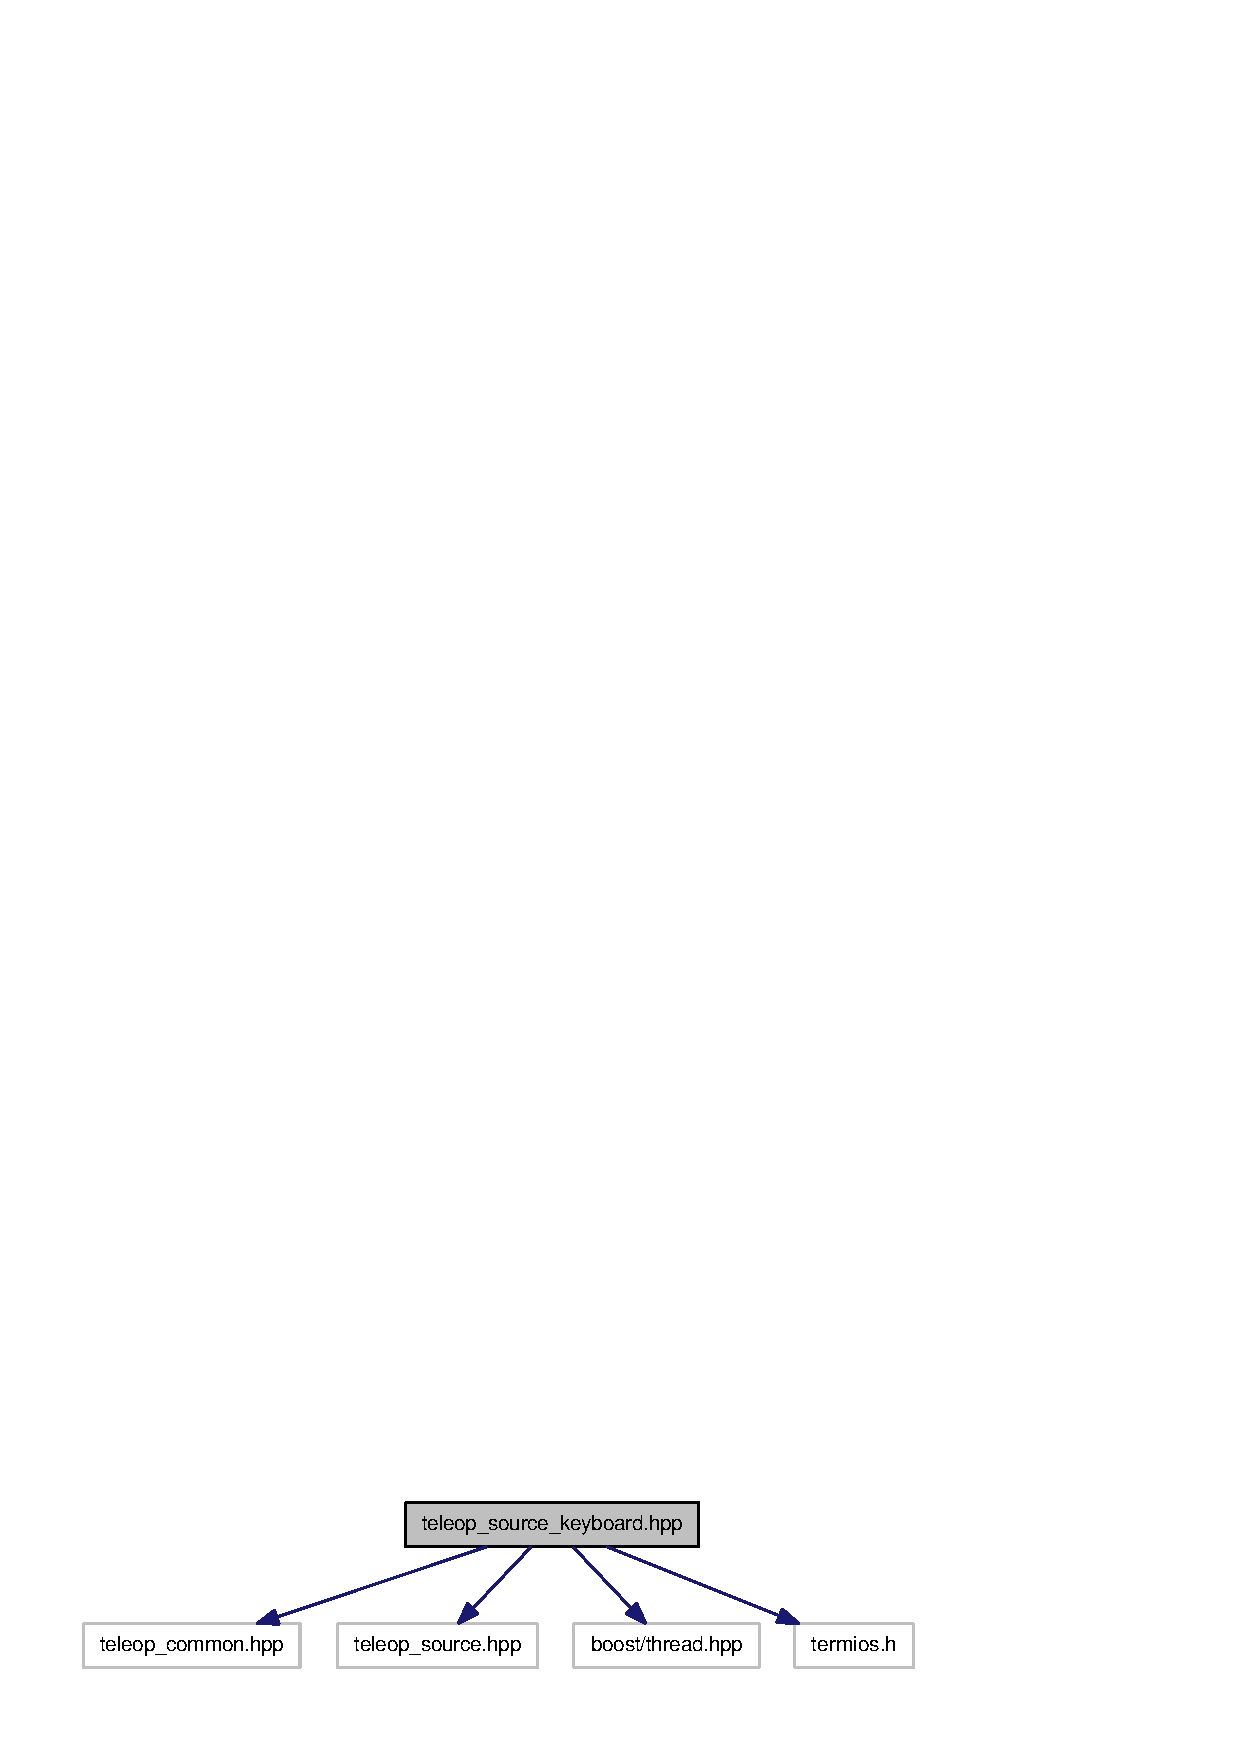
\includegraphics[width=400pt]{teleop__source__keyboard_8hpp__incl}
\end{center}
\end{figure}
This graph shows which files directly or indirectly include this file:
\nopagebreak
\begin{figure}[H]
\begin{center}
\leavevmode
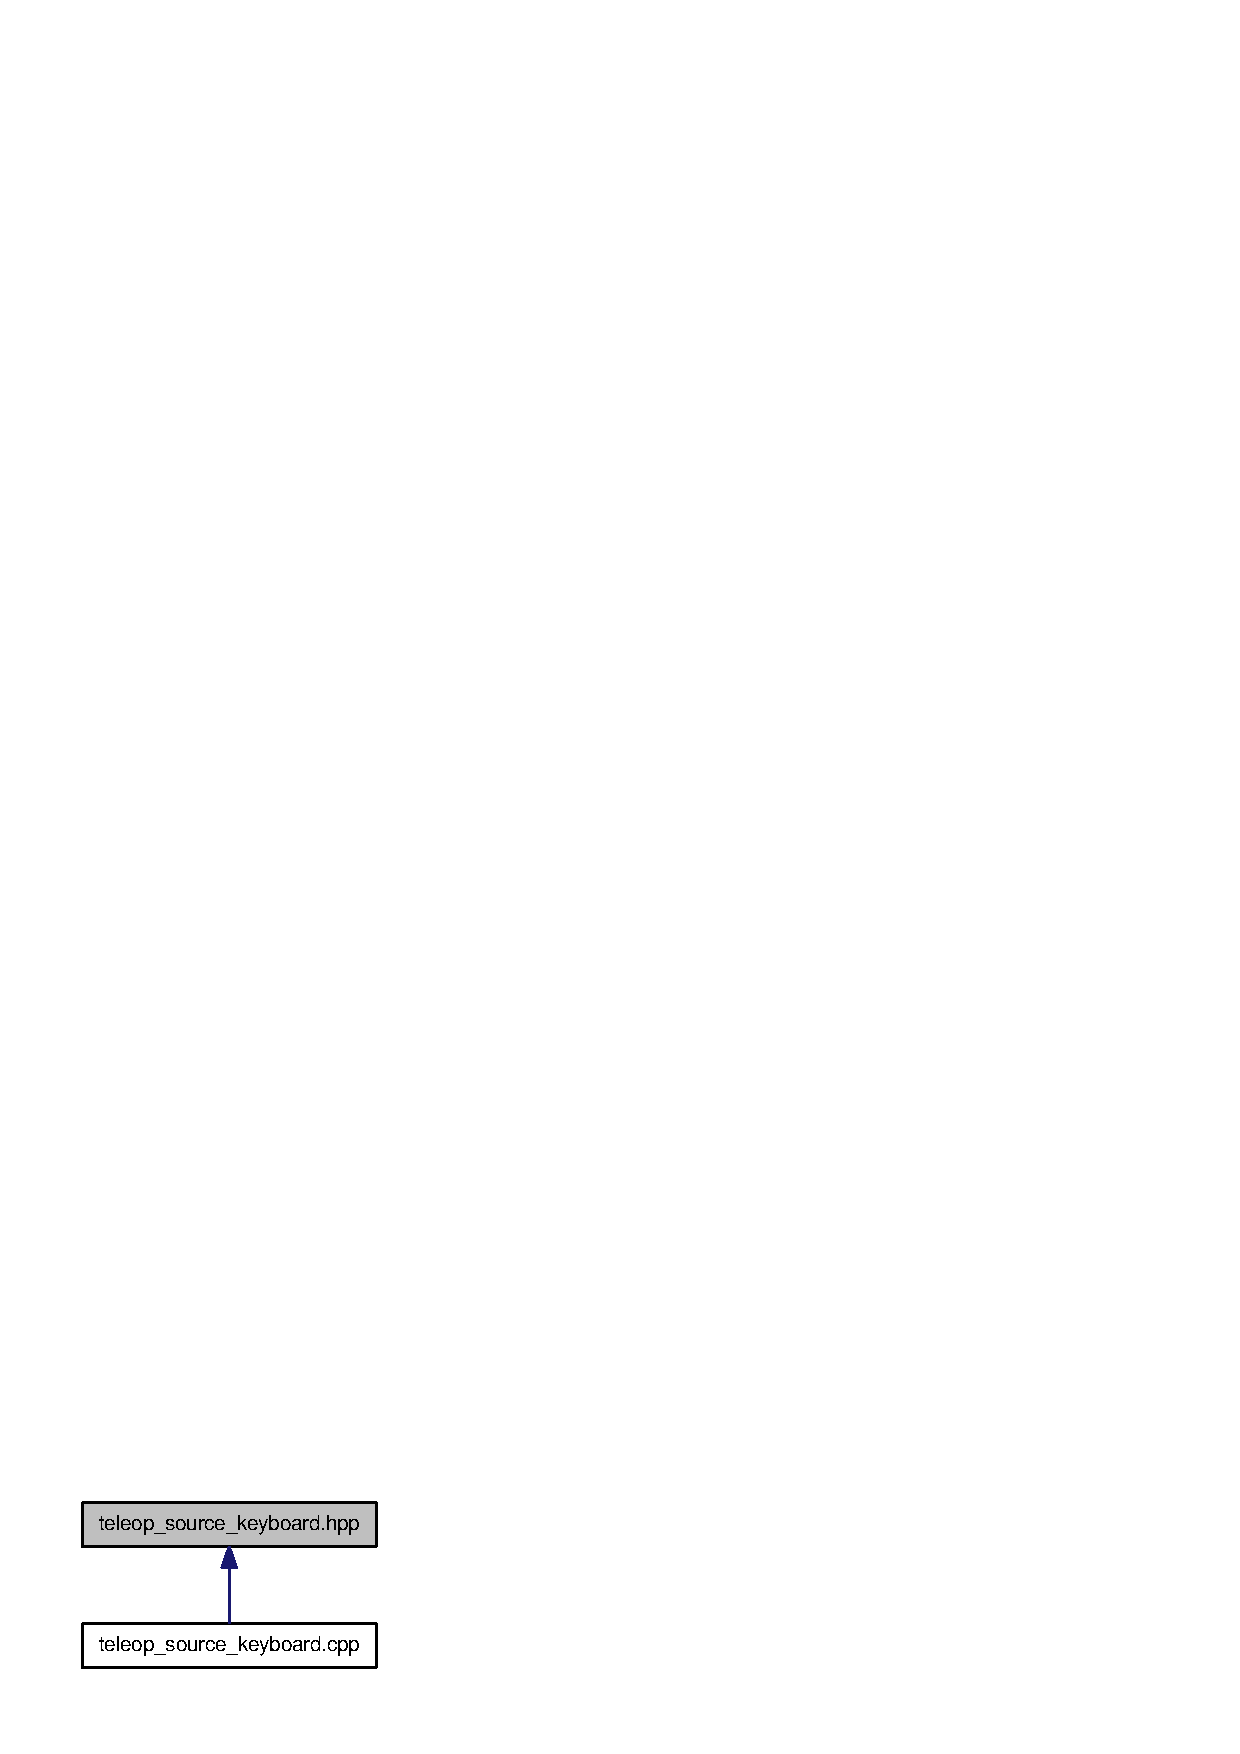
\includegraphics[width=400pt]{teleop__source__keyboard_8hpp__dep__incl}
\end{center}
\end{figure}
\subsection*{Classes}
\begin{DoxyCompactItemize}
\item 
class {\bf teleop::TeleopSourceKeyboard}
\end{DoxyCompactItemize}
\subsection*{Namespaces}
\begin{DoxyCompactItemize}
\item 
namespace {\bf teleop}
\end{DoxyCompactItemize}

\section{/home/klc/Code/github.com/teleop/teleop\_\-msgs/mainpage.dox File Reference}
\label{mainpage_8dox}\index{/home/klc/Code/github.com/teleop/teleop\_\-msgs/mainpage.dox@{/home/klc/Code/github.com/teleop/teleop\_\-msgs/mainpage.dox}}

\section{/home/klc/Code/github.com/teleop/teleop\_\-source\_\-keyboard/src/teleop\_\-source\_\-keyboard.cpp File Reference}
\label{teleop__source__keyboard_8cpp}\index{/home/klc/Code/github.com/teleop/teleop\_\-source\_\-keyboard/src/teleop\_\-source\_\-keyboard.cpp@{/home/klc/Code/github.com/teleop/teleop\_\-source\_\-keyboard/src/teleop\_\-source\_\-keyboard.cpp}}
{\ttfamily \#include $<$teleop\_\-common.hpp$>$}\par
{\ttfamily \#include $<$teleop\_\-source.hpp$>$}\par
{\ttfamily \#include $<$teleop\_\-source\_\-keyboard.hpp$>$}\par
{\ttfamily \#include $<$boost/thread.hpp$>$}\par
{\ttfamily \#include $<$sys/select.h$>$}\par
{\ttfamily \#include $<$termios.h$>$}\par
{\ttfamily \#include $<$unistd.h$>$}\par
{\ttfamily \#include $<$time.h$>$}\par
{\ttfamily \#include $<$stdio.h$>$}\par
Include dependency graph for teleop\_\-source\_\-keyboard.cpp:
\nopagebreak
\begin{figure}[H]
\begin{center}
\leavevmode
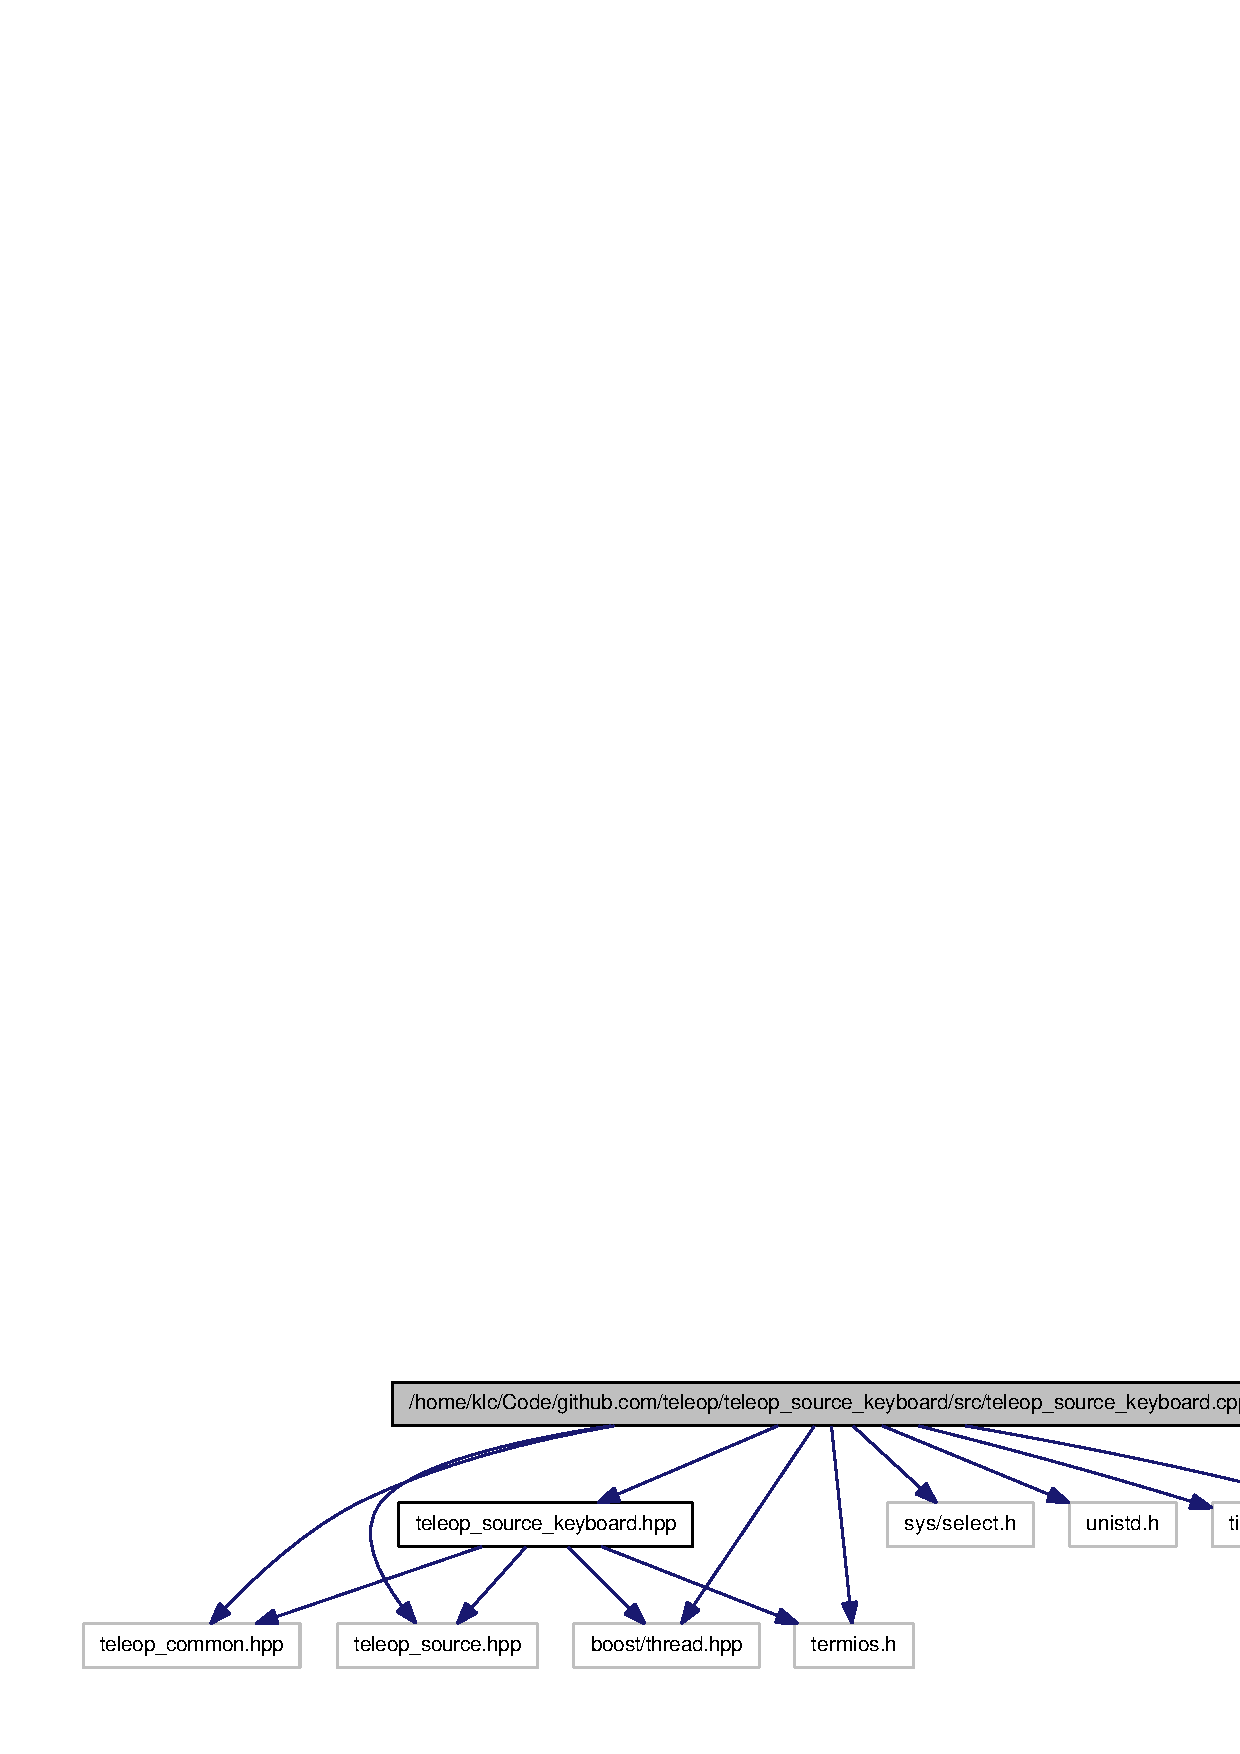
\includegraphics[width=400pt]{teleop__source__keyboard_8cpp__incl}
\end{center}
\end{figure}
\subsection*{Namespaces}
\begin{DoxyCompactItemize}
\item 
namespace {\bf teleop}
\end{DoxyCompactItemize}

\printindex
\end{document}
